\documentclass[../main.tex]{subfiles}

\begin{document}
	\section{Sound}
	\begin{preamb}
		Sound is transferred in a form of a wave. In this chapter we will explore the different properties of sound and some of its applications.
	\end{preamb}	
	\subsection{Fundamentals}
	Some fundamental properties of sound:
	\begin{itemize}
		\item Sound is produced by a vibrating source.
		\item Sound exists in the form of a longitudinal wave.
		\item In different media, sound has different speeds. Generally, the higher the density, the faster the speed of sound.
	\end{itemize}
	\begin{center}
		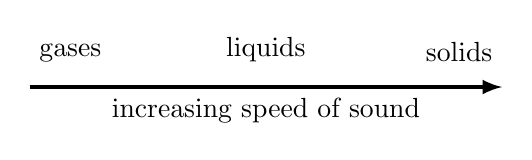
\begin{tikzpicture}
			\draw [line width=0.5mm, -latex] (-3,0) -- (3,0) node[anchor=north, pos=0.5 ] {increasing speed of sound};
			\node [anchor=south west] at (-3,0.2) {gases};
			\node [anchor=south] at (0,0.2) {liquids};
			\node [anchor=south east] at (3,0.2) {solids};
		\end{tikzpicture}
	\end{center}
	\peqn{Speed of Sound}{For a sound source from \(d\) away from an observer and capturing it after a time \(t\), the speed of sound can be calculated as}{v = \frac{s}{t}}
	
	\subsection{Properties of Sound}
	\peqn{Loudness}{The loudness of a sound wave is directly proportional to the square of its amplitude}{\text{loudness} \begin{cases}
			\text{louder} &\text{higher \(A\)} \\
			\text{softer} &\text{softer \(A\)}
		\end{cases}}
		
	\peqn{Pitch}{The pitch of a sound is directly proportional to its frequency}{\text{pitch} \begin{cases}
			\text{higher} &\text{higher \(f\)} \\
			\text{lower}  &\text{lower \(f\)}
		\end{cases}}
		
	The human ear can hear sounds from between \SI{20}{\hertz} to \SI{20}{\kilo\hertz}.
	
	\subsection{Applications of Sound}
	\pdef{Echo}{An echo is the repetition of a sound due to the reflection of sound.}
	Echo is used in distance measurement systems such as SONAR in ships. 
	
	\pdef{Ultrasound}{Ultrasound is sound with frequencies above the upper limit of the human range of audibility (i.e. \SI{20}{\kilo\hertz}).}
	Ultrasound is used in product quality control and pre-natal scanning.
\end{document}
